%%% The main file. It contains definitions of basic parameters and includes all other parts.

%% Settings for single-side (simplex) printing
% Margins: left 40mm, right 25mm, top and bottom 25mm
% (but beware, LaTeX adds 1in implicitly)
\documentclass[12pt,a4paper]{report}
\setlength\textwidth{145mm}
\setlength\textheight{247mm}
\setlength\oddsidemargin{15mm}
\setlength\evensidemargin{15mm}
\setlength\topmargin{0mm}
\setlength\headsep{0mm}
\setlength\headheight{0mm}
% \openright makes the following text appear on a right-hand page
\let\openright=\clearpage

%% Settings for two-sided (duplex) printing
% \documentclass[12pt,a4paper,twoside,openright]{report}
% \setlength\textwidth{145mm}
% \setlength\textheight{247mm}
% \setlength\oddsidemargin{14.2mm}
% \setlength\evensidemargin{0mm}
% \setlength\topmargin{0mm}
% \setlength\headsep{0mm}
% \setlength\headheight{0mm}
% \let\openright=\cleardoublepage

%% Generate PDF/A-2u
\usepackage[a-2u]{pdfx}

%% Character encoding: usually latin2, cp1250 or utf8:
\usepackage[utf8]{inputenc}

%% Prefer Latin Modern fonts
\usepackage{lmodern}

%% Further useful packages (included in most LaTeX distributions)
\usepackage{amsmath}        % extensions for typesetting of math
\usepackage{amsfonts}       % math fonts
\usepackage{amsthm}         % theorems, definitions, etc.
\usepackage{bbding}         % various symbols (squares, asterisks, scissors, ...)
\usepackage{bm}             % boldface symbols (\bm)
\usepackage{graphicx}       % embedding of pictures
\usepackage{fancyvrb}       % improved verbatim environment
\usepackage{natbib}         % citation style AUTHOR (YEAR), or AUTHOR [NUMBER]
\usepackage[nottoc]{tocbibind} % makes sure that bibliography and the lists
			    % of figures/tables are included in the table
			    % of contents
\usepackage{dcolumn}        % improved alignment of table columns
\usepackage{booktabs}       % improved horizontal lines in tables
\usepackage{paralist}       % improved enumerate and itemize
\usepackage{xcolor}         % typesetting in color
\usepackage{enumitem}
\usepackage{refstyle}		% easy image referrencing
\usepackage{hyperref}
\usepackage{float}

%%% Basic information on the thesis

% Thesis title in English (exactly as in the formal assignment)
\def\ThesisTitle{Natural Language Generation system writing football articles}

% Author of the thesis
\def\ThesisAuthor{Dan Raffl}

% Year when the thesis is submitted
\def\YearSubmitted{2022}

% Name of the department or institute, where the work was officially assigned
% (according to the Organizational Structure of MFF UK in English,
% or a full name of a department outside MFF)
\def\Department{Institute of Formal and Applied Linguistics}

% Is it a department (katedra), or an institute (ústav)?
\def\DeptType{Institute}

% Thesis supervisor: name, surname and titles
\def\Supervisor{RNDr. Jiří Hana, Ph.D.}

% Supervisor's department (again according to Organizational structure of MFF)
\def\SupervisorsDepartment{Institute of Formal and Applied Linguistics}

% Study programme and specialization
\def\StudyProgramme{Computer Science}
\def\StudyBranch{General Computer Science}

% An optional dedication: you can thank whomever you wish (your supervisor,
% consultant, a person who lent the software, etc.)
\def\Dedication{%
Firstly, I would like to thank my supervisor \Supervisor  for his valuable advice as well as his support. Secondly, I am grateful to every teacher I had the chance to meet at Faculty of Mathematics and Physics for their attitude and inspirational work. Last but not least, I would like to thank my family for supporting me throughout my studies.
}

% Abstract (recommended length around 80-200 words; this is not a copy of your thesis assignment!)
\def\Abstract{%
Journalism could become a tedious job as its main concern is to create as many articles as possible, usually prioritising quantity over quality. Some articles are quite routine and they need to exist just because most of the population prefers text over raw data. The idea is to ease this job and generate articles, particularly about football in Czech language, automatically from non-linguistic data. 

This thesis is concerned with analysing implementation of such a linguistic software and moreover offers a brief overview of a Natural Language Generation (NLG) process. The major focus of this overview is on benefits and drawbacks of different approaches to NLG as well as describing NLG tasks and its challenges you need to overcome in order to produce a similar human language (not only Czech) producing program. 
}

% 3 to 5 keywords (recommended), each enclosed in curly braces
\def\Keywords{%
	{NLG}, {Czech}, {sport}, {football}
}

%% The hyperref package for clickable links in PDF and also for storing
%% metadata to PDF (including the table of contents).
%% Most settings are pre-set by the pdfx package.
\hypersetup{unicode}
\hypersetup{breaklinks=true}

% Definitions of macros (see description inside)
\include{macros}

% Title page and various mandatory informational pages
\begin{document}
\include{title}

%%% A page with automatically generated table of contents of the bachelor thesis

\tableofcontents

%%% Each chapter is kept in a separate file
\chapter*{A - Introduction}
\addcontentsline{toc}{chapter}{Introduction}

Charles Babbage, the father of the computer, had the first impulse for the invention of a mechanically calculating system at college, when he was tired of mistakes in a table of logarithms. He suggested constructing a machine powered by steam, which could process a larger number of computations than humans while avoiding making mistakes. The idea of using computers to our advantage is carried even now in a highly-paced competitive technology-driven world. Even in the field of journalism, computer science has advanced and the results are getting quite stunning. In 2020  well-known British newspaper The Guardian published an article titled “A robot wrote this entire article. Are you scared yet, human?” \cite{gpt32020robot}, in which AI language generator GPT-3 explains why its existence is not a threat to the existence of mankind. Ignoring the main point of the article, it is well written and I doubt that anyone would recognize that humans did not write the text. Furthermore, in 2022 GPT-3's abilities to write fluent prosaic text were described equivalent to that of a human by The New York Times \cite{johnson2022ai}. This proves the results of AI in the field of language generating.

In this article we discuss numerous challenges of generating text in general and how to conceptually approach developing a language-producing software. This process of generating text (or some linguistic output as discussed below) is in the field of computational linguistics referred to as Natural Language Generation or NLG. These challenges are explained using various specific examples to illustrate exactly what may cause problems and how to prevent them. Also the aim of this paper is to introduce different techniques on how a NLG system can be organised and approached. Everyone who reads the paper should then be able to construct a solution for a NLG problem and especially be aware of the strengths or weaknesses of the solution.

Furthermore, one specific implementation of NLG is presented along with its analysis. This analysis includes description of overall structure, specification of how individual tasks are approached and finally a discussion of the solution. The task fully specified in Chapter (TODO - A - doplnit číslo kapitoly) was to generate a brief article that summarises what happened in a football match. To avoid ambiguity, throughout the article the word "football" refers to a sport, which American English speakers call soccer. This is a first neat example of detailed aspects you need to be aware of when developing a NLG system - meaning of a word can change with different locations. Therefore, it is very important to know the target audience of the generated language. 




\chapter{A - Natural Language Generation}

\section{A- What is NLG?}
The intuitive meaning of the Natural Language Generation (NLG) is rather obvious, unlike the definitions that usually vary. I will now present definitions of NLG by two different authors:
\begin{enumerate}
	\item “NLG is the subfield of artificial intelligence and computational linguistics that is concerned with the construction of computer systems that can produce understandable texts in English or other human languages from some underlying non-linguistic representation of information.”\label{win-1}\cite{reiter1997building}
	\item “Natural Language Generation (NLG) is the process by which thought is rendered into language.”\label{win-2}\cite{mcdonald2010natural}

\end{enumerate}

The  definition (\ref{win-2}) is much broader and less reliant on specification of what is output and especially input of such a task, which is here defined as “thought”. The problem of identifying the source has been discussed even earlier in \cite{mcdonald1993issues}. He compared the situation to human conversation, namely when the speaker starts deciding what to say. Then the source can be state of mind, current situation, speaker’s intentions etc. These inputs are bordering on the impossible to classify and represent in a computer. The output is defined simply as language, without any stress on the representation of the language. On the other hand, the definition (\ref{win-1}) defines output as understable text, which implies the form of the result is written and additionally restricts the input to be non-linguistic data. However, in the article authors also mention that their survey is focused on written texts, but the principles could be also applied to generating spoken language, which implies the definition could be extended. Examples shown above, and especially the contrast of specifying what output or input can or can not be, explain why it is extremely hard to define the term NLG precisely. 
Let us consider the problem of summarising a book into a brief description. Given this problem and definitions above, we can see that it satisfies only the second vague definition, since the input is purely linguistic. This kind of problem is referred to as text-to-text generation. An example of such a generation is extracting summary from a dialogue of a customer and customer service department described by \cite{liu2019automatic} or pun generation \cite{ritchie2005computational}.
 
Similarly, the initial problem can be transformed into video-to-text generation by switching a book with a movie. In this scenario the line blurs even more. A movie has two components - sound and the video itself. The video has implicitly some semantic meaning and is surely non-linguistic. Howerever, the sound usually contains spoken language and therefore is linguistic. For instance, a video shows Mark pointing at an apple and the sound is “This is a pear.”. The sound itself implies there is a pear, but the message could be summarised as Mark is lying or Mark is not able to recognize a fruit. Finding a correct summarization would be impossible with one of the components missing, because they both affect the overall message, which makes deciding if video-to-text could be classified as NLG difficult. This logic of reasoning can be applied to other problems that vary in their initial inputs such as generating diagnostic report from image (e.g. roentgen) by \cite{zeng2020generating}, which could be characterised as image-to-text generation.

In this article, NLG is perceived as described by \cite{reiter1997building}, meaning creating text from non-linguistic data. This task is often referred to as data-to-text generation. Examples given throughout the article will fit this definition and the idea in general. Methods and approaches mentioned in this article may presumably be applied to any problem concerned with computational linguistics if it is suitable without a need to classify the problem as NLG.

\section{A - Usage of NLG}
The aim of the NLG is to generate documents, articles, messages, emails, descriptions and other forms of texts in order to either reduce workload or to offer a customer a user-friendly interpretation of data in a given language. Various sources papers offer data-to-text implementations operating with different domains, input data and overall aims of the language (which can differ as well):
\begin{itemize}
	\item summarising data and creating reports 
	\begin{itemize}
		\item summarising statistics from a baseball match \cite{puduppully2022data}
		\item summarising geo-referenced data such as map \cite{thomas2007atlas}
		\item creating textual weather forecasts \cite{sripada2014case}
		\item creating report of student's academic performance \cite{}
	\end{itemize}
	\item creating poetry (e.g. in Finnish by \cite{hamalainen2018harnessing})
	\item producing text to persuade reader something is good or bad \cite{carenini2006generating}
\end{itemize}
The most common usage of NLG is to summarise less readable data to more convenient textual form regardless of the domain (sports, weather, geography, etc.). Even though the output of these two tasks is the same, the reason to apply the NLG system is different - compare textual weather forecasts to reports of a student's academic performance. Weather reports are produced in order to enable the general public to find out information about weather since their ability to interpret meteorological raw data is probably lacking. Same reason appears when summarising baseball statistics and maps. On the other hand, there is no doubt that teachers and professors can correctly interpret grades from student’s studies, but the problem is to do that as quickly as possible as well as obtaining the data in a well-readable layout. Generating textual summary automatically resolves both issues effectively at the same time.

The summaries and reports do vary in one more important aspect - the amount of the information and level of terminology. For instance, when creating a weather report for everybody to read some information such as type of the rain or concrete number of mm will not be mentioned in the output text and the information will be abbreviated to “heavy” rain since this is the information the reader is interested in. Contrastingly, when creating a medical report (e.g. from surgical procedure) the terms should be precise and technical (possibly in latin) and the amount of information left out is close to minimum. To conclude, the target audience and their knowledge of the domain will alter the produced text substantially.

The overall aims of the language diverge significantly. In producing poetry the rhymed text filled with phrases calling forth emotions is used to achieve experience as powerful and captivating as possible when reading it. In summaries the aim is to convey the factual information to the reader in an easy and understandable way. Notice that this should be a significant aspect of choosing an approach for the problem. If the goal of the text is to inform, then text is highly recommended to be as simple as possible. On the other hand, if the aim is to captivate, as it is in newspaper articles, then creating simple dull sentences is not a suitable option. 

This was the first glance into the aspects that are crucial when deciding how to approach a language generating problem. These aspects are mentioned many times across the text since the goal of this article is to present to the reader how to approach the NLG and the correct understanding is one of the key parts to develop a solid NLG system.

Is the NLG system good to use every time? Debate whether the software is worth creating is indeed viable and maybe a little underestimated since the articles usually do not analyze feature elaborately. In the real world this is a question of economic resources. Wages and time saved on the human work that has been replaced with software must outweigh the cost of the creation and maintenance of the software. Easy examples of evidently beneficial usage of NLG system is customer service emails generator. Even a simple inserting name to the start of the email, then stating the product, order number and a little survey of satisfaction with the product is quite a trivial email to generate, does the job and saves tons of company time. Possible example of a non-optimal usage is when text is not the most convenient form of data for the user to comprehend. Charts, tables, schemata, maps or pictures could be considerably easier to transfer the intentional message to the end user as these structures are usually attractive and intuitive\footnote{Combination of visual representation of data and text could also be the best alternative in a certain scenario.}. To give you an example, imagine coloured map of a city and using a red line to highlight the path to the nearest tourist information centre in comparison with text composed of verbal instructions where to go. Obviously, map is a better solution due to its simplicity and visuality. 


\chapter{NLG Tasks}\label{chap:tasks}
Transforming non-linguistic data into grammatically correct sentences in a given language seems like a rather complicated problem. Therefore it is convenient to divide the initial problem into smaller tasks, which are easier to solve. This task structure is described by \cite{reiter1997building} and it is widely used to cover every challenge a fundamental NLG problem should deal with:
\begin{itemize}
	\item Content determination
	\item Discourse planning
	\item Sentence aggregation
	\item Lexicalization
	\item Referring expression generation
	\item Linguistic realisation
\end{itemize}

In this section we will discuss every task mentioned above. Note that approaches, which will be described later, may change this structure: there might be just a few changes by combining multiple steps and processing them simultaneously or the structure may be completely decomposed. Moreover, using data-driven methods is dominant approach and can be utilized across every task of the NLG. Their usage will be omitted in this section and further closely discussed in \autoref{chap:approaches} taking the uniqueness and dissimilarity of this approach into consideration.

The reason we describe every task individually is to highlight challenges that will arise along the way of creating the NLG system. Understanding these tasks is a crucial aspect to produce a well-built software regardless of the choice of the approach. To illustrate the problems we state numerous simple examples that should ease the process of fully recognizing the extent of issues related to each task.

\section{Content determination}
The goal of this task is to decide what information from input data should be included in the text. Usually the range of the input data is significantly larger than the amount of information we would actually transfer to the user. Naturally, this task is heavily influenced by the specifications of the assignment, namely domain, intention of the text and target audience. Consider the problem of creating a medical report from a complete blood count for a patient to read. This domain requires data preprocessing to recognize negative indicators from values contained in test results. In addition, a doctor or expert is needed to assist in order to interpret values correctly and set rules on how to identify diagnosis. The goal of the text is to describe the diagnosis in an understandable way and therefore using Latin or overly technical terminology should be avoided. However, if we take the doctor as a target audience, we now want to use the as precise expert language as possible and probably change the content to present segments of the test results and not just the overall diagnosis to enable the doctor to better interpret marginal symptoms or flag values.

The result of the content determination is usually outputted as a set of preverbal messages, carrying semantic meaning of the statement. To carry all the information an implementation that can describe abstract concepts such relations between statements, entities or conditions is needed. This sub-task of creating suitable representation is usually domain-dependent. Since the important semantic information is mapped into some formal language, there is no need for (human) language to be specified, and therefore this task is language-independent. Concrete examples of formal representation language used to store these semantic attributes are for instance logical language, attribute-value matrices or graphs.

Example of the result of possible content determination is shown below in \figref{cd}, where we would like to choose the content to report one simple message: a goal being scored in a football domain. We have two related (3) sets of attribute-value pairs: (1) is about a player and (2) contains goal statistics. Obviously some information in tables (1) and (2) are too specific (e.g. height of the player) for the message to convey and therefore redundant. Bold attribute-value pairs are highlighted as the ones to be present in the final text, creating preverbal message (4) in pseudocode, which is an output of content determination task. After performing the remaining NLG tasks possible result could look like (5). 

\begin{figure}[h]
	\centerline{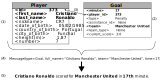
\includegraphics[width=0.9\textwidth]{./img/content_determination.pdf}}
	\caption{Process of content determination}
	\label{fig:cd}
\end{figure}

\section{Discourse planning}
Previous part determines what messages will be transmitted to the reader and this part resolves the issue of the order in which the information is presented. This process is also referred to as text or document structuring. Selecting the right sequence of messages is crucial for text to accomplish its goal. Similarly we structure academic texts to logically ordered paragraphs, which present the topic in a way as understandable as possible for the reader to gain knowledge.

Similarly to content determination this task is highly domain-dependent as we have to know how to order messages. For instance, a medical report (as an example mentioned earlier) would likely display diagnoses and order decreasingly by how dangerous and life threatening they are. On the other hand, a report from a business meeting could start with a brief overview of achievements and goals and then with issues that were discussed ordered chronologically to allow the reader to follow the course of the meeting.

Human brain orders information to be conveyed in a speech intuitively, but the process as an algorithm itself is not quite trivial. Most of common method is to create rules based on the specific domain since the suitable structure heavily relies on the domain. Some researchers suggest using machine learning techniques for creating a  uniform algorithm independent of the domain as seen in \cite{dimitromanolaki2003learning}.

Form of the output of discourse planning can differ. One possible option as described by \cite{reiter1997building} is a tree structure. Leaves of the trees are messages and inner nodes describe specifics of their function in a sentence. This may seem like an unnecessary complicated solution when clustering messages to be said in one sentence can be just an array of messages. The benefit of the tree structure is the amount of information we can store along the messages including constraints under which the message can be said, relations between them and their overall structure.

\section{Sentence Aggregation}\label{section:sa}
The cardinality of the relation message and sentence is rarely one-to-one. Usually multiple messages are formed into one sentence. This process is called sentence aggregation and it is fundamental for generating text that is readable and flows well. To clarify we provide set of verbal messages:
\begin{enumerate}
	\item \emph{Peter bought an apple.}\label{sa-one}
	\item \emph{Peter bought a banana.}\label{sa-two}
	\item \emph{Anne did not buy anything.}\label{sa-three}	
\end{enumerate}

This set of sentences is clearly non-optimal and can be aggregated in two steps as follows:\footnote{\label{footnote-opt}Naturally, no such concept as "optimal" sentence exists. The optimum in this case is to express the information in a sentence that would likely occur in a spoken human language and also would appear fluid and natural.}
\begin{enumerate}[resume]
	\item \emph{Peter bought an apple and a banana. Anne did not buy anything.}\label{sa-four}
	\item \emph{Peter bought an apple and a banana, whereas Anne did not buy anything.}\label{sa-five}	
\end{enumerate}

We can notice two types of aggregation leading to the optimal sentence (\ref{sa-five}). Aggregation of:
\begin{itemize}
	\item \textbf{constituents} - Constituents that have equal syntactic importance can be aggregated using suitable coordinating conjunctions expressing their relation. Take example sentences (\ref{sa-one}) and (\ref{sa-two}). \emph{Apple} and \emph{banana} are both items \emph{Peter} bought so their semantic meaning is identical. Therefore they can be aggregated via cumulative conjunction \emph{and} creating a new noun phrase in the result sentence (\ref{sa-four}) \emph{an apple and a banana}. Another example of cumulative conjunctions is \emph{both ... and} or \emph{as well as}.
	\item \textbf{sentences} - Sentences can be aggregated as well using coordinators as seen in the result sentence, which was created by inserting an adversative conjunction in between sentences in example (\ref{sa-four}) to express opposition. This contrast can be expressed by other words like \emph{but}, \emph{yet}, \emph{while}, etc. More relations can be expressed when aggregating sentences using another kinds of coordinating conjunctions: \emph{alternative} (\emph{or}, \emph{either ...or}, \emph{nor}) to express two or more alternatives and \emph{illative} (\emph{for}, \emph{so}) to express interference or consequence.
\end{itemize}

One more type of aggregation can occur based on explicit hand-crafted domain-based rules. Take these three preverbal messages from football domain reporting a goal, which are similar to the one as used in \figref{cd}-(4) (Manchester United shortened to MU):
\begin{enumerate}[resume]
	\item \emph{(type=Goal, full\_name="Cristiano Ronaldo", team = "MU", time = 4)}\label{sa-six}	
	\item \emph{(type=Goal, full\_name="Cristiano Ronaldo", team = "MU", time = 8)}\label{sa-seven}
	\item \emph{(type=Goal, full\_name="Cristiano Ronaldo", team = "MU", time = 14)}\label{sa-eight}	
\end{enumerate}

Surely realising messages (\ref{sa-six}), (\ref{sa-seven}) and (\ref{sa-eight}) as three different sentences would not create fluid and natural results as sentences would vary only in time of the goal. Since three goals in football form a so called hat-trick we could aggregate messages in one sentence:
\begin{center}
	\emph{Cristiano Ronaldo completes hat-trick for MU in under 15 minutes.}
\end{center}

This aggregation realises the messages (\ref{sa-six}, \ref{sa-seven}, \ref{sa-eight}) beautifully as the result is well-formed and natural. Notice that the aggregation happened also in expressing the time of the goals: instead of mentioning three different timestamps the time is summarised as "under 15 minutes" highlighting the fact that this rare figure was achieved in a short amount of time. As described in the previous section, domain knowledge is necessary to decide what is "long", "short" or "average" (and therefore not worth mentioning) amount of time for an event to happen.

Note that these aggregations are simple for humans, but to perform them in a NLG we need some semantic knowledge and relations of the sentences (or constituents). The easiest approach is to define domain-specific constraints when to perform aggregation. Defining complex domain-independent rules and universal representation of relations is rather a difficult task and nowadays often solved using data-driven methods, which are described later in \autoref{chap:approaches}. 

Furthermore, the idea that the more aggregations we perform the better the final text is wrong. Sometimes slowing down the flow of information by fracturing the message into smaller individual sentences is useful in order to produce more understandable text. Overloading sentences can often result in less fluency as the more information is conveyed in one sentence the harder it is for a reader to follow. \cite{barzilay2006aggregation} are perceiving this as a linear programming problem where similarity is classified for each pair of database entries. Using this similarity, transitivity and global constraints (e.g. maximum number of aggregation across the document) they find an optimal solution.   

\section{Lexicalization}
After performing discourse planning and sentence aggregation the preverbal messages are in a correct order and they contain suitably aggregated information. Goal of this task is to create mapping from these messages to specific expressions in a given human language. This task is the first that is language-dependent. There are two main problems associated with lexicalization. Firstly, the amount of combinations of how to narrate a message is enormous, only restricted to those that fit into the given context. And secondly, transformation of concept into a word (or more words) is very abstract and interferes with many layers of the language (semantics, phonetics and pragmatics) and therefore choosing a suitable expression is rather difficult. This transformation is not even easy for humans. Imagine an essay contest in grammar school with a given topic of the essay. If the transformation was easy and had only one solution, the contest would not exist as essays would be identical. In fact, the perspective and overall understanding of the topic, style of describing one’s point of view and finally even choosing words to present the idea is partly what distinguishes us as people. 

Another factor is the target audience and the overall goal of the language. If the target audience is educated on the matter then using adequate technical terminology is reasonable. Contrastingly, for low-skilled readers all terminology must be explained in an easy way and the content of the text should be more about overall ideas rather than about specific concepts. 

Trivial approach to this task is to hand-craft pairings of a word or a whole phrase and a concept in a message. This solution results in monotonic outputs as the aspect of choice is missing. Slight improvement would be to add more semantically similar options for each item. However, this can cause problems. First of them is how to decide, which possibility is the best. Second is the possible non-viable combinations of words together. One example, that may be not visible on the first glance, is generation of adjectives interpreting numbers. For example, take a person with height 185 cm. If it was a man, the height is "average", while a woman could be described as "tall". Therefore semantic background and suitable comparison need to be taken into account. What is more, combinations of chosen phrases may result in non-realisable or simply weird expressions. 

Due to the vagueness and coherence of the process, NLG systems combine lexicalization, REG and linguistic realisation under one operation called surface realisation or tactical part of the process.  

\section{Referring expression generation}
Referring expression generation (REG) is a process, when you choose words to express domain entities or other constituents of the message. Naturally, utilising one noun phrase for one specific entity, which is used more than once in a short amount of text, results in less readable and fluid text. On the contrary, there is a limit to how many such expressions we can generate since a reader needs to identify the entity correctly. Ambiguity is a highly unwanted effect since the information that needs to be conveyed may differ from its actual language semantic meaning.

To fully understand the challenges and also possible solutions for REG here is an example of sentence where we would like to lexicalize its subject represented as an entity in pseudocode:
\begin{center}
\emph{(entity=Country, name=”Czech Republic”) has a population of 10,3 million.}
\end{center}
This particular country can be lexically expressed in this sentence for example as:
\begin{enumerate}
	\item \emph{Czech Republic} \label{reg-1}
	\item \emph{Czechia} \label{reg-2}
	\item \emph{Country nicknamed “The heart of Europe”} \label{reg-3}
	\item \emph{Bohemia, Moravia and Czech Silesia} \label{reg-4}
	\item \emph{Country in the central Europe} \label{reg-5}
	\item \emph{Country which borders Germany, Poland, Slovakia and Austria} \label{reg-6}
	\item \emph{Beautiful rustic country in the heart of Europe} \label{reg-7}
	\item \emph{It} \label{reg-8}
	\item \emph{This country} \label{reg-9}
\end{enumerate}
Notice the linguistic techniques we used to express this subject:
\begin{itemize}
	\item \textbf{Entity name} - Using the name of the entity is a trivial solution and works fine as seen example (\ref{reg-1}).
	\item \textbf{Synonyms} - Using a synonym or a different name having the identical semantic meaning for the entity as shown in example (\ref{reg-2}) and (\ref{reg-3}). 
	\item \textbf{Descriptive transcription}  - using the knowledge of physical appearance, characteristics or its location we can describe an entity without any need of using its initial name. Examples (\ref{reg-5}), (\ref{reg-6}) and (\ref{reg-7}) are all using the location in Europe. Although expression (\ref{reg-6}) identifies Czechia unambiguously, the description of the location may be too specific for a less-educated reader (or possibly for a reader living outside of Europe), who has no idea where Germany is. The information that the country is situated in Europe is then sufficient. Therefore the target reader, his knowledge about a topic and also the purpose of the text are important even in this task. This technique is also prone to ambiguity as seen in example (\ref{reg-5}): reader should already know what country is described in the text to use this expression since more countries can be characterised as “central European”.
	\item \textbf{Definite descriptions} - The expression can be enriched by adding valid adjectives, adverbs or other linguistic structures to further specify the object as seen in example (\ref{reg-7}) where adjectives rustic and beautiful describe the country even a little bit more creating enriched and complex noun phrase.
	\item \textbf{Pronouns} - In a human language pronouns are often used to represent entities (e.g. “I have seen him.” or examples (\ref{reg-8}), (\ref{reg-9})). Using pronouns correctly can help to improve readability of the text and also minimise the obvious flags of computer-generated text. The main obstacle to overcome is when to use pronouns. Sometimes usage of a pronoun can arise from context, sometimes if there is absolutely certainty that everyone knows what the pronoun is referring to: those examples are hard to deal with and usually handled explicitly. Usual approach is to use pronoun if the entity was mentioned in a previous sentence under the condition the entity was the only constituent the pronoun could refer to.
\end{itemize}

How to approach REG depends also on repetition of the entities in the text and the final text variability. In a domain where identifying the entity unambiguously is primary (e.g. city in air travel) the usage of REG is even harmful. For instance, expressing "New York, USA" as "The city that never sleeps" in the air travel domain. To the contrary, expressing an entity identically multiple times in a short span of prosaic text eventuates in dull, plain and stereotypical language. 

\section{Linguistic realisation}\label{section:lr}
This task transforms every constituent to form a grammatically and syntactically well-built sentence. Example of a struggle when building even a simple noun phrase is:
\begin{enumerate}
	\item \emph{(entity=Animal, name =”dog”, count=1) $\rightarrow$ one dog} \label{lr-1}
	\item \emph{(entity=Animal, name=”dog”, count=23) $\rightarrow$ 23 dogs} \label{lr-2}
	\item \emph{(entity=Animal, name=”mouse”, count=2) $\rightarrow$ two mice} \label{lr-3}
	\item \emph{(entity=Animal, name=”fish”, count=1000) $\rightarrow$ thousand fish} \label{lr-4}
\end{enumerate}

Trivial and also naive solution for this simple noun phrase building can be to append morpheme “s” to the name of the animal if the count is more than one. As you can see in example (\ref{lr-3}) and (\ref{lr-4}) this solution can work only for animals that have regular plurals. In addition, the count itself is recommended to be expressed by a word and not by numeral if the number is either a small integer (1-10) as seen in the comparison of  examples (\ref{lr-1}) and (\ref{lr-2}). Same rule applies as well for a well-known rounded number (hundred, thousand, billion, etc.) shown in (\ref{lr-4}).

One, so far omitted important, aspect is the principles of morphology and syntax of the language. Concept of appending morpheme "s" to express plural might not be so easily transferable into different languages. In Slavic languages morphemes to express plural differ and also can be infixed, meaning they could be inserted into the word stem instead of using a suffix. In Czech, a word for dog is \emph{pes}. Then realising their number would look like: \emph{1 pes, 2 psi, 5 psů}. To further complicate the situation, Slavic languages are fusional. That means a single morpheme carries multiple grammatical, syntactic or semantic meanings. In Czech, agreement between the grammatical case and the noun is resolved as well with an infix morpheme. Here are three examples in Czech using different grammatical cases along with translation from English:

\begin{itemize}
	\item (case: nominative) \emph{two \textbf{dogs}	$\rightarrow$ dva \textbf{psi}}
	\item (case: genitive) 	\emph{without two \textbf{dogs}  $\rightarrow$ bez dvou \textbf{psů}}
	\item (case: instrumental) \emph{with two \textbf{dogs} 	$\rightarrow$ s dvěma \textbf{psy}}
\end{itemize}

Notice that not only the noun, but the word for number 2 (\emph{dva}) as well are subject to the linguistic transformation as the infix morpheme carries both the agreement with case and the plural. 

We have mentioned typology according to morphology (fusional language). Another type is analytic languages (e.g. Vietnamese), where every single word is exactly one morpheme. Lastly, the complete opposite is polysynthetic languages (e.g. Inuit languages), where one word is constructed by combining plenty of morphemes representing a whole sentence. In central Nunavut Inuktitut \emph{Tusaatsiarunnanngittualuujunga} means \emph{I cannot hear very well}. 

The extent of language influence is huge even in the semantic part as well. To demonstrate, imagine generating a sentence, in which the action will happen in the future. This may seem like a trivial problem in English since we may just use the word "will" (or other modals). However, English, unlike Romance languages (French, Spanish, Italian and more) does not have future grammatical tense. Some languages are even tenseless, e.g. Tokelauan spoken in American Samoa (Polynesia). This section just illustrated the need for the knowledge and principles of the language during the linguistic realisation.  

Realisation has quite an extensive magnitude caused by the non-trivial goal of correctly morphologically and syntactically (as well as semantically) expressing each of the lexical items in the sentence. This process requires adding auxiliary words (prepositions, verbs, etc.), handling agreements, ordering,  inserting punctuation and other similar transformations all in order to present the language not only factually, but even grammatically right. Due to the complexity of the task multiple approaches exist. One of them is using templates. 

\textbf{Templates} are hand-crafted using fixed lexical items and attributes substituted in the template. Preverbal message (\ref{lr-t-1}) is assigned to a template (\ref{lr-t-2}) and three variables are then substituted with values creating the target sentence (\ref{lr-t-3}). 

\begin{enumerate}
	\item preverbal message $\rightarrow$ Message(type=Goal, full\_name = "Cristiano Ronaldo", team = "Manchester United", time = 17) \label{lr-t-1}
	\item template $\rightarrow$ \textbf{\$full\_name} \emph{scored for} \textbf{\$team} \emph{in} \textbf{\$minute}\emph{th} \emph{minute}. \label{lr-t-2}
	\item result $\rightarrow$ \textbf{Cristiano Ronaldo} \emph{scored for} \textbf{Manchester United} \emph{in} \textbf{17}\emph{th} \emph{minute}. \label{lr-t-3}
\end{enumerate}

The advantage of this approach is simplicity and prevention of grammatical errors considering that we have full control of what the fixed segments are and any unwanted error is highly improbable. The disadvantages prevail. First of all, applying templates could be only feasible in well-defined low-volume domains as entities must be have easy-to-text-interpretation. Another reason is that creating templates is time-consuming. And most importantly, the variation of the output is low as the immutable parts of the text generate very limited output. In addition, the template approach for more complicated languages tends to struggle, because the constituents usually depend on each other (e.g. agreement, auxiliary words, etc.) creating requirements that are hard to fulfil. 

However, templates are extremely practical when the target output is expected to be simple and 
rarely changing. Great example is generating spoken announcements in the transportation domain e.g. departures of flights on the airport, where the template could look like: \emph{The departure of flight number \$number from \$destination\_from to \$destination\_to will be slightly delayed. $\rightarrow$ The departure of flight number FD-2018 from Rome to Paris will be slightly delayed}. Results are admittedly blunt in terms of language richness, but they are factually correct, clear and easy to comprehend, which was the initial purpose.
     
Other approaches are more complicated in order to outperform templates in a range of expressions.  First of them is building a grammar for the natural language. This approach relies on thorough knowledge and examination of the language behaviour and principles offering domain-independent solutions that can be applied to a different NLG system performing linguistic realisation. The advantage of this approach is definitely the domain independence of the realiser as well as its variety in produced output. Disadvantage is that building such grammar is labour-expensive and the disability to select the best possible result. All generated sentences will be correct, but the choice, which one is the optimal one is beyond grammar's reach.

Secondly, data-driven (further described \autoref{chap:approaches})methods can be applied in this task too. However their usage can vary greatly. Both approaches above can be enhanced by these stochastic methods since we can reduce manual workload. Templates can be automatically extracted from training corpus (more about corpora in \autoref{chap:process}). Similarly, hand-crafted grammars can be created automatically from corpora. Also, linguistic approaches can be avoided by using these methods. However, fusing traditional linguistic approaches and the power of statistical approach can result in a well-performing system. For instance, using hand-crafted grammar in combination with stochastic methods to resolve the optimal-among-the-correct-ones issue.



\chapter{NLG approaches}\label{chap:approaches}
We will divide approaches based on two aspects:
\begin{itemize}
	\item Structure of solution
	\item Methods used in a solution
\end{itemize}	

Note that we can fuse structure and methods arbitrarily in our desired solution. 

\section{Structure of solution}
So far we have covered what individual tasks we need to cover in our solution without suggesting a proper structure, which organises these tasks together and creates a compact implementation. There are two main approaches:
\begin{itemize}
	\item \textbf{Modular architecture} -- This architecture uses a pipeline of modules. Often this architecture follows the design suggested by \cite{reiter1997building}, with each module corresponding to one or more tasks they suggest (see \ref{chap:tasks}). 
	\item \textbf{Global approach} -- The tasks are fully deconstructed and the problem is solved globally in order to get rid of the limitations associated with modular architecture. 
\end{itemize}

\subsection{Modular architecture}\label{section:modules}
This approach was described by \cite{reiter1997building} and became almost a standard for a long time. The idea is to construct a module for each NLG task and link those modules via a one-way pipeline. Hence, output of content determination is an input for discourse planning and so forth. But some of the tasks are closely related and therefore it is efficient to assign those tasks to one module. Accustomed layout by \cite{reiter1997building} of modules is: 
\begin{itemize}
	\item Text (document) planner -- content determination + discourse planning
	
	= \emph{``what to say”}
	\item Sentence planner -- sentence aggregation + lexicalization + REG
	
	= \emph{``how to say it”}
	\item Linguistic realiser
	
	= \emph{``saying it correctly”}
\end{itemize}

Text planner determines the content of the text as well as the order, in which we present the content to the reader. This part of the NLG process is also referred to as strategic generation. Sentence planner transforms messages from text planner to a lexicalized expression. And finally linguistic realiser combines these expressions with regard to syntactic and grammatical rules of given language. Choices made during sentence planning and linguistic realisation are often together called, on the other hand, tactical. Clear distinction between tactical and strategic will be more important later when discussing data-driven methods.

The main advantage of this 3-module is the structure itself, which is easy to follow and understand. In addition, offering clear division of what is each module’s obligations as well as what issues they do not resolve. Simplicity results in accessible and well-structured code. Moreover, it is easier to change a minor functionality of the program since classifying where to change the code is intuitive. The same logic applies for methods used across the solution: one or more tasks can be approached completely differently than the rest of the code using other methods (e.g., statistical) while keeping the input and output formats of each module.

However, the strict sequentiality of the architecture is also its main drawback. Once we decide sentence order and content we have no chance of changing it later and so the choices in the early stages may later result in an unsolvable issue. Imagine generating a sentence with a limited maximum number of characters. In a text planner we have chosen the content of the sentence, but even when we do every possible combination of lexicalization of the sentence the number of characters still exceeds the upper bound. So what now?! The solution would be to retroactively change the content of the sentence and drop part of the initial information, but this is not possible since the pipeline is one sided. Of course this problem could be bypassed by making the pipeline go backwards, but this would completely break the principle of modular approach. The clear line of division among modules would disappear and modules' functionality and objectives would suddenly overlap. 

\subsection{Global approach}
Assembling the structure of the text before knowing linguistic resources may result in incorrect, ambiguous or bizarre expressions. Therefore global approach is based on breaking the crisp division of the modular structure and alternating between different NLG tasks depending on the state of the development and the constraints that arise along the process while having full context available at all times. This is the core idea of the approach, however, how to implement similarly working solution differ hugely. One example of such implementation, that can be formally described, is planning.

\subsection{Planning approach}
In order to produce a text in a decent quality many decisions must be made resulting in various alternatives. Similarly as described in \cite{fikes1971strips} where the idea is to find a universal robot solver for the world model represented as first-order predicate formulas. The broadness and vagueness of the process of starting with various preconditions and getting to the desired result lead to planning.

Planning problem (as well as planning approach in general) is described by \cite{gatt2018survey} as ``the process of identifying a sequence of one or more actions to satisfy a particular goal”. Actions are then described as preconditions and their effect after applying them. In the terms of NLG, the goal is to convey the message along with its aim (persuade, inform, captive, …) to the target person. The actions then have constraints under which they can be performed and the effect is the change to the current context all leading to the desired goal of the language. The main idea is to create formalism that does not rely on a strict structure of the NLG system and available solutions to alternate between different NLG tasks with the recognition of both current state and effects of the chosen actions all in order to create the best possible language and broaden the limits of pure modular approach. 

\section{Methods}
After we specified how to compose a solution, we propose methods and approaches to use in a chosen structure of the solution. In \ref{chap:tasks} we proposed  methods mostly using structures and formalisms (e.g., templates or grammars) that are based on the linguistic knowledge of the language. However, even in \ref{chap:tasks} we mentioned data-driven methods that can be incorporated to solve a particular NLG task. Data-driven (or statistical,  stochastic) methods are a widely discussed topic among the NLG community as their popularity grows and their results are recently getting better, often outperforming more traditional procedures. Therefore the whole next subsection is dedicated to them. 

\subsection{Data-driven approach}
As the name implies, data-driven methods crucially rely on data, which consist of inputs and corresponding outputs. Using statistical or probabilistic principles of comparing our current state of the NLG process to a similar state in the data ensures making choices similar to those in the training dataset. In the field of linguistics this data is referred to as corpus. Since these methods can be applied on even smaller segments of the generation data can contain processed input or output data in various internal representations, which appear during the process and not just the initial and final stage. For example, when computing sentence planner inputs of our testing data are preverbal messages and outputs are lexicalized texts.

The very first obstacle that arises when performing these methods is the acquisition of the input-output data, because the data must fulfil some requirement. The amount of the dataset should be big enough to ensure the validity and overall principal of the statistical and probabilistic approach. The dataset must not only satisfy the requirement on the quantity, but certain variety must be ensured as monotonic data tend to give one-sided and misleading results. 

Acquiring data itself can be tricky. Easiest scenario when an already established corpus for a specific domain (e.g., weather forecasting, hotel and restaurant recommendation, sport reports and more) exists. These corpora are well-built, but on the other hand useful only when working with the same domain. The reason for that these corpora may be available is firstly because their usage is common and secondly for their input data simplicity. Working with a less-common domain with larger range, types or complexity of data will result probably in the absence of a viable corpus and therefore building the corpus is another problem appended to the NLG process. To overcome this problem we can either build a new corpus from scratch or exploit more stochastic methods that automatically align input with outputs. Then again one disadvantage is that the data are heavily domain-specific. The alignment of the input to the segments of output is crucial for most of the methods except deep neural networks and other machine-learning methods. These methods are recently becoming dominant in certain subfields of NLG such as image-to-text generation.

After assuming we have acquired data for the full-ranged NLG process, we can classify a stochastic approach based on the overall architecture. One group approaches the problem globally and completely decomposes the modular approach in order to both avoid error propagation and allow the software to make decisions freely across multiple tasks and different stages of generation. In opposition, the second group upholds at least the division between tactical and strategic choices.  

We state some examples to further illustrate usage of data-driven approach with different specific methods and range of NLG process they cover:
\begin{enumerate}
	\item \textbf{stochastic process} - Work of \cite{ratnaparkhi2000trainable} is a nice first example to introduce data-driven methods, because he described three systems (NLG1-3) along with their comparison. Systems are used for tactical generation (semantic context is provided in a corpus given attribute-value pairs aligned with textual outputs) in an air travel domain. First system (NLG1), for given attributes, simply chooses a template with the highest number of occurrences in the training data. Second system uses a maximum entropy probabilistic model to predict the best proceeding  word taking the already generated and also the attributes yet to be generated into account. However, the dependency of the words in language may not come from their order. Therefore NLG3 predicts the best words based on their syntactic relations represented by a tree. Along with the system's description \cite{ratnaparkhi2000trainable} offers their results in terms of correctness. Both NLG2 and NLG3 heavily outperformed NLG1. Furthermore, NLG3 was performing slightly more accurately than NLG2.  \cite{ratnaparkhi2000trainable} states that both NLG2 and NLG3 can be used in other domains as well, but the complexity of the domain must be somewhat similar to the air travel (meaning quite low). Implicitly domain annotated data must be provided to further exploit NLG2/3 systems.\label{dd-1}
	\item \textbf{classification} - \cite{duboue2003statistical} used classification process in their system for automatic content determination illustrated on biography generation problem. System is provided with initial data and target texts. Algorithm starts with clustering the semantic data (e.g., by age) and matching segments of the output to the pieces of input. This forms a solid base for the process of creating content selection rules using the binary classifier for each attribute of input data whether the attribute should be mentioned or not.\label{dd-2}
	\item \textbf{optimisation} - The article of \cite{marciniak2005beyond} researches the optimisation process in Natural Language Processing (NLP) approached as an integer linear programming problem. They use this approach even in a field of NLG when generating textual route directions. The global approach results in the elimination of error propagation and has better overall results as a consequence according to \cite{marciniak2005beyond}. Summary of the specifics such as the metric that should be minimized during linear programming is further described, for instance, in \cite{gatt2018survey}).\label{dd-3}
	\item \textbf{probabilistic context-free grammar (PCFG) and parsing} - The idea of mixing the NLG tasks together is further exploit by \cite{konstas2013global} as they call the division of every single task separately ``greedy". The need for domain-specific approach is here eliminated as this work is concerned with concept-to-text generation. They use input to model a PCFG and then use the stochastic methods to acquire the best word sentence satisfying the grammar. Such a process can be viewed as an opposite to semantic parsing. This system was tested on three different domains: sportscasting, weather forecasting and air travel query generation. Performance results were described as same or even better to the methods known at the time.\label{dd-4}
\end{enumerate}
Note that these four examples not only show various specific statistical methods, but they illustrate other nuances as well. Take the range of the process they cover for instance. Examples (\ref{dd-4}) and (\ref{dd-3}) cover end-to-end process, contrastingly example (\ref{dd-2}) covers only the tactical part and example (\ref{dd-1}) only covers content determination. Moreover (\ref{dd-1}) and (\ref{dd-2}) keep the strategic and tactical division unlike (\ref{dd-4}) and (\ref{dd-3}). Domains differ as well, especially in example (\ref{dd-4}), in which domain does not have to be specified.

These examples share two more similarities except the implicit statistical approach. Firstly, they rely heavily on the testing data and especially their alignment of input and output. Secondly, their results are somewhat superior to other hand-engineered systems. Often hand-crafting a NLG system relies heavily on the domain and lacks portability and certain variability of the output (respectively achieving the variability by hand is the more tedious job the more variable the output should be). NLG systems grounded on statistics are robust and a task of data acquisition is added to the end-to-end solution. This is counterbalanced by good (or even better results as described, for instance, in \citet{konstas2013global} more portability as example (\ref{dd-4}) is domain-independent. These methods along with the solid linguistic foundation are nowadays dominant \citep{gatt2018survey} since the robustness is not big enough to be uncomputable with modern computers and the availability  and amount of testing data is much higher. 
\chapter{Process of developing an NLG system}\label{chap:process}

The process of developing a text-producing software is complex and requires organised preparation in order to deliver a quality result. This paper so far covered separate segments of the NLG accompanied by numerous examples to illustrate concrete problems. Now we suggest how to order key parts of the development:
\begin{enumerate}
	\item Requirements analysis \label{p-1}
	\item Corpus building \label{p-2}
	\item Choosing suitable architecture and approaches \label{p-3}
	\item Implementation of the NLG system \label{p-4}
	\item Evaluation \label{p-5}
\end{enumerate}

Steps (\ref{p-1}), (\ref{p-2}) and (\ref{p-5}) are further discussed in separate sections below. Steps (\ref{p-3}) and (\ref{p-4}) were already described in detail in \autoref{chap:tasks} and \autoref{chap:approaches}. Both steps (\ref{p-2}) and (\ref{p-5}) are skippable and not required, but their implementation can further enrich the final solution.

\section{Requirements analysis}

First step of developing the NLG system is to carefully analyse fundamental aspects that will establish the approach and overall functioning of the program. We state six such aspects:
\begin{itemize}
	\item Input data
	\item Expected output
	\item Target language
	\item Goal of the language 
	\item Target audience
	\item Usage of already existing tools  
\end{itemize}

Examples in the article were created to demonstrate the various effects these aspects could have. This section will briefly summarise nuances that can occur. 

\textbf{Input} data can have different inner representations: table, database, graphs, images, etc. Furthermore data can be in its initial state and probably will require some preprocessing to, for instance, extract computable information or transform data into better structured and more suitable other representation. Some representations can result in creating non-trivial tools to extract needed information for the generation, e.g. image requires image recognition software.

\textbf{Expected output} can be specified in corpus (described below). Knowledge of desired output is key to analyse the full extent of other aspects.

\textbf{Target language} can as well influence the approach greatly, especially the solution for the tactical part of the program. In the section about linguistic realisation (\autoref{chap:tasks}) we have covered some differences between languages. Naturally, deeper linguistic analysis is required to fully recognize the specifics of the language and how to approach lexicalization, REG and realisation. Moreover, the NLG system can generate identical messages in multiple different languages and then the approach for the solution can be restricted to only those that strictly divide tactical and strategic choices.

\textbf{Goal of the language} is very important as seen in examples throughout the article. For instance, producing a routine text with formal requirements will be approached differently than generating an eye-catching book teaser.

\textbf{Target audience} has a couple of characteristics: age, literacy rate, level of education or knowledge of the domain and topic. These details should be taken into consideration in order to deliver the message to the reader in the most convenient and understandable way possible. 

Lastly, a great number of \textbf{already existing tools} has been developed and it is a possibility to incorporate these tools into newly constructed solution. Examples can be domain specific corpora or specific language realisers. Utilising these already established resources can upgrade the solution. However, the negative impact of such usage can be making ponderous transformations to create input in correct form that is required by the incorporated system as well as accommodating the approach to the tool.
 
\section{Corpora building}
As we mentioned above, requirement factors can greatly influence methods and our overall approach to the problem. Communicating these specifics can be tricky when only one side has an insight into computational linguistics. The most suggested method is to create a corpus, which is a collection of inputs and corresponding text outputs. This process ensures a clear definition of expectations of what the output will look like and prevents misunderstanding. This method is useful even when developing software independently without any specific party, that would require any specifics. Corpus is then built to our own expectations creating a solid base for the process of approach analysis and implementation of the NLG system in general. 

Additionally, corpus is necessary when applying statistical methods since they rely completely on the content of the corpus and the correlation in-between. Lastly, corpus does not have to be composed of end-to-end NLG pairs, but rather contain inputs and corresponding outputs for a smaller part of the NLG (one or more tasks) in order to create a foundation for stochastic methods to resolve the problem. Inputs and outputs can then vary greatly in the inner representation as for instance inputs for content determination and REG will surely differ. What is more, since data structures  alter even for the same NLG task solution the corpus should be built (or transformed) so that the input and output fit the specific solution's representations.

Hand-building a corpus from scratch should be supervised and consulted with a domain expert (e.g. for creating medical reports the doctor should participate in creating example texts) in order to achieve the best result possible. For corresponding input an example output should be written by a domain expert. The result of this process is called an initial corpus. The developer should now make a revision of the initial corpus to guarantee that the NLG system can deliver the expected text, because not every input and corresponding output must necessarily be feasible. Firstly, the output text can be improved (e.g. when acquiring texts from existing one). Secondly, the information that is contained in the sentence may not be present nor computable from the given input data.\footnote{The information can also be somehow contained in the initial data, but building tools for its extraction would be insanely time consuming or the time complexity of the extraction would be high and therefore not possible: this is up to the developer to analyse and determine data transformations within his reach.} This is a critical part of the development as there is no way to resolve this problem every time and it is highly application-dependent. Common solutions are to extend the input data or remove unavailable information from the text and create a new version avoiding the information. Similarly, a compromise of finding hand-formed rules when to convey the information may be the solution. After all the necessary changes to the initial corpus were made, the corpus is now composed strictly of well-built and agreed upon example texts, where every information needed to its generation is contained in a data directly or it can be computed from given data. This finalised corpus is called target text corpus.

What should a good corpus look like? Corpus should be comprehensive and offer a wide range of pairs input-output. Edge cases, exceptions or less unusual texts should be incorporated in the corpus as well as average text to produce. Naturally, the number of normal texts to produce should be significantly higher than the number of rare examples to indicate the correct ratio. Corpus should be exhaustive in terms of expectations: once the corpus is finished, adding functionality explicitly is very complicated and is likely to change the overall structure, depending on its complexity. 

Described process of hand-building corpus is highly labour-expensive and therefore usually domain-dependent systems for automatic acquisition of the data are developed lately further exploiting the strengths of statistical methods in combination with the amount of accessible data. Some NLG problems can find better results when extracting output texts from already existing “approved” texts. For example, when generating a short weather forecast it would be ineffective to create newly-written texts. Much better approach would be to extract forecasts from the most popular weather websites and take those as expected outputs. Benefits of this approach are reduced time spent acquiring example outputs and also ensured quality of the text since using popular websites. Some downsides could arise when applying this approach: acquiring this data can contradict with copyright law and range of the input data can differ resulting in unavailable knowledge. Also the output text of our new implemented NLG system (when done optimally) will produce similar texts as those popular websites and therefore there is no reason why our forecast should become more read and popular than the already existing ones. This approach is suitable when the domain content will probably be very similar, reducing the amount of knowledge that may be unavailable. On top of that, the number of available output texts must be high to make use of the stochastic approach. Such domains are weather forecasts, sport reports or the (air) travel domain and more.

To summarise, building a corpus is not obligatory, but highly recommended practice to ease the process of developing the NLG system, especially finding requirements. Precise target corpus primarily precedes the problem that the quality of the developed system is insufficient as the user knows exactly what the output will look like and match his expectations perfectly. When applying statistical methods, a well-defined and comprehensive corpus becomes a necessity since the stochastic approach relies crucially on the power of data. Lastly, the corpus is a fine tool even for the developer himself: analysis of each record of the corpus results in an outline of the challenges to overcome and gives a basic idea how the particular NLG problem should be approached.

\section{Evaluation}
After NLG yields the textual result an intuitive action would be to rate it and then reflect the approach and implementation based on the rating. From a practical point of view this step can be processed by a user or client who expects a certain quality and decides whether the quality is matched or not. From an academic point of view, this task is about deciding how to measure what is the "optimal" output as described in footnote \ref{footnote-opt}. Computer science problems usually contain a metric, which easily decides what solution is better. For instance, graph problems usually have an optimal solution to the problem and algorithms are compared based on time complexity of finding this optimal solution.\footnote{Exceptions are probabilistic and approximation algorithms that find acceptable (compared to the optimal) solution in a faster time} However, in linguistics the comparison metric is not obvious, but rather complicated.

This can be demonstrated in a school-leaving essay. Deciding about the grade will likely be uniform since the base is some general criteria that have to be matched. However, how to decide what work was the best (if the goal was to pick the best essay). Surely, we can restrict ourselves to only the theses that were graded with the best grade, but how to choose among them? To summarise, in linguistics it is trivial for a human to decide if the result is "good" or "bad", but it is difficult to pick the best among the "good" ones. "Bad" results can be grammatically incorrect, factually wrong or the communicative goal was not achieved. This process is even harder for computers and therefore a human element is often required to rate the results. 

It seems that the measure tools differ very much from what to measure to how to to measure it. Readability, fluency, and correctness can be viable attributes rating the linguistic appearance of the text. What information is present in the text, how it is presented to the reader, whether the information is relevant and if the communicative goal was achieved are attributes to grade content of the text and the overall vibe. Grading these attributes can be then approached alternatively as well: by grading on discrete or continuous scale, ordering texts or simply picking the best text in a given aspect. The metric should be designed to reflect important aspects for the given texts.

The uncertainty of this step is predictable as the importance and consequences of small nuances in the texts are interpreted subjectively. \cite{gatt2018survey} recommend aiming for diversity in the approach to yield a wide range of results and then decide the best final approach based on not only the results, but on the correlation between them as well.


\chapter{Implementation}

In this chapter we will take a close look into the overall functioning of an football articles generating NLG system. The goal was to create an end-to-end NLG system, that takes non-processed raw data about a football match as an input and creates article in Czech language that summarises the development of a match. The aim of the thesis was not only to get the basic understanding of a NLG process, but also try to create the implementation in a language that is widely used around the world and for me, personally, was less known - Python.

\section{Requirements and initial goal}
As mentioned in the introduction of this section, the expected output was simply a readable Czech text summary while attempting to produce sentences that are not identical resulting in less-monotonic text. Since the expected output was defined as somewhat vague and quality-wise uncertain, there is no stress on the definition of goal of the language and target audience. However, the text quality, especially in the variability of expressions, used structures and overall richness, is insufficient to truly satisfy the definition of an article. 

Since NLG is a complex process we used one already existing tool for linguistic realisation - \emph{Geneea API}. Without this tool the output language would not be grammatically correct and therefore not satisfying the readability requirement. As discussed in (TODO-A-ref na linguistic realisation) this task has no easy way of implementing manually, especially not for a Czech language that belongs to the most complicated natural languages (for reasons that are described in (TODO-A-ref na linguistic realisation)). \emph{Geneea API} usage skips this task focusing on the rest of the NLG tasks combined.

In \autoref{chap:process} (TODO - A - ref a whole section) We proposed an outline to a requirements analysis. This section will follow this structure describing the specifics.

\section{Input data}
Dataset was provided by a company Livesport s.r.o. (TODO-A-mám ji zmiňovat), which I would like to thank. Therefore entire dataset can not be shared. However, one example match is attached to illustrate program functioning. Initial dataset is composed of every match of one Czech First League season. Every match is represented as JSON file storing both general information about the match (teams, venue, attendance, line-ups, etc.) and course of key events of the matches (goals, substitutions, cards, etc.). 

General information about the match consists of two participating teams, starting time of the match, tournament information (here it is Czech First League for the particular year), information about venue, score, winner, stage of the game (e.g. finished/delayed) and line-up. Line-up consists of every player of the team divided into groups according to their status (e.g. injured, benched, initial line-up, etc.) among with other information like home country, number and more. 

Course of events is represented as a list of incidents. Incident has attributes like id, time, participant, type and so on. Also, incidents have attribute \emph{parentId}, which further specifies the incident. For instance incident type \emph{Penalty Kick} has empty \emph{parentId}, however, in incidents there is incident type \emph{Penalty Scored} or \emph{Penalty Missed} that has \emph{parentId} identical to corresponding \emph{Penalty Kick} \emph{Id}. 

\section{Approach}

For this NLG problem I have chosen modular architecture as described in (TODO-A-ref section) - the most traditional, even though now a little outdated, approach proposed by \cite {reiter1997building} consisting of grouping similar NLG tasks into modules that are then connected via one-way-pipeline. 

In the first place, I would like to highlight the reasons that led to a chosen approach:
\begin{itemize}
	\item My personal lack of experience in NLG as this was my first ever NLG system that I have created.
	\item The lack of easily accessible big amount of data.
	\item The full extent of a NLG problem - from non-processed data to well-built text.   
\end{itemize}

For me, personally, this field of computational linguistic is new and therefore the aim  was not only to build a NLG system, but gain knowledge including different approaches in this specific subfield of NLP. Staying faithful to the division of modules is the most intuitive and also feasible solution, which closely relate to the point of the end-to-end extent of the problem. It was easy for me to get lost in the high amount of issues to resolve (each of the NLG tasks) without giving it a properly divided structure. Also the error propagation was another problem that has risen from the lack of experience.

In addition, the lack of data almost forbids the data-driven approach. Naturally, the data do exist, but their acquisition would require either high amount of time consuming labour of creating the data by hand or developing football articles automatically and then aligning them with given input data, which still can end up insufficient as for the acquired text more data could have been known. Such a corpus building could be a project on its own.

\section{Match example}
A match example is provided and the summary can be seen in \figref{overview}. 

Football match between \emph{Jablonec} and \emph{Bohemians 1905}, which resulted in a 3 to 1 victory for the home team \emph{Jablonec}. First half can be summarised in words to further describe the figure: First goal was a penalty scored by \emph{Trávník} in 10th minute and then second incident was a goal by \emph{Bohemians'} player \emph{Hašek} that tied the game in 44th minute after a pass from \emph{Vaníček}. Events that happened in second half are hopefully easy to interpret as well. Numbers next to a incident group them by their type- (1) penalty goal, (2) goal with an assist, (3) substitution and (4) yellow card. 

\begin{figure}[p]
	\centering{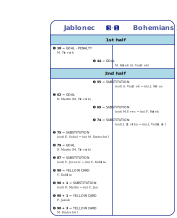
\includegraphics[width=0.9\textwidth]{../img/match_overview.pdf}}
	\caption{Table summary of the example match.}
	\label{fig:overview}
\end{figure}

\section{Structure overview}
The overview of the structure of the solution is shown in \figref{structure}.

Input data with arguments to modify slight functioning (as way of output, or number of texts to generate) are passed to \emph{run.py} (\figref{structure} - 1) (.py will be left out as it is implicit for every module), which is the executable starting point of the program. Parsed arguments are an input for \emph{articles\_generator}, which handles the communication between each module, essentially creating the one-way-pipeline for modules (\figref{structure} - 2, 3, 4, 5) and managing passing the suitable inputs and outputs. Output of this core handler is tuple of strings - title and body of the article.

The \emph{data\_initializer} (\figref{structure} - 2) is as module not present in the original module architecture by \cite{reiter1997building} (described in (TODO-A-odkaz na sekci)). However, since the data is in a raw form, the step of data processing needed to be added to store the data in a more convenient way to further operate with the information given.

Modules (\figref{structure} - 3, 4, 5) correspond to the modular architecture perfectly. \emph{Document\_planner} (\figref{structure}-3) takes data about a match in a convenient inner representation. Creating a \emph{DocumentPlan}, which contains preverbal messages to be said in a sentence. Then these messages are lexicalized in \emph{sentence\_planner} (\figref{structure} - 4) and finally linguistically realised by \emph{linguistic\_realiser} (\figref{structure} - 5). 

Moreover, there are three auxiliary modules to keep the structure of the implementation as clean as possible:
\begin{itemize}
	\item \emph{Data.py}
	\item \emph{Types.py}
	\item \emph{printer.py}
\end{itemize}
These are further described later in (TODO-ref).

\begin{figure}[p]
	\centering{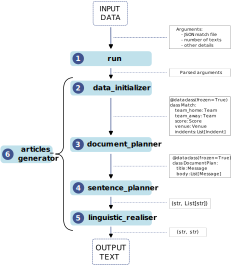
\includegraphics[width=1\textwidth]{../img/program_structure.pdf}}
	\caption{Overview of solution structure.}
	\label{fig:structure}
\end{figure}

\section{Modules implementation}
In this section the implementation of each module is described in detail creating a compact solution in Python. I

\subsection{Auxiliary modules}
\textbf{\textit{Data.py}} groups data classes that store information contained in a JSON file. Namely these entities are \emph{Score, Venue, Country, Player, Team, Time, Incident (+IncidentParent) } and finally the most crucial \emph{Match} that encapsulates each of the class mentioned. Note that these classes are made immutable using \emph{@dataclass(frozen=True)} from package \emph{dataclasses} and then implementing static \emph{create} method. Immutability ensures the data remain intact after manipulating with them frequently in multiple functions across modules. 

Module \textbf{\textit{printer.py}} manages printing different components in a readable way. Since there is a lot of data, even during the development it was more convenient to pretty-print separate results of modules instead of inspecting more nested and complicated states during debugging. Due to numerous alignments and length of string appending separate module was created to not overload other segments of the code.

Lastly, \textbf{\textit{Types.py}} stores enumarate types for different entities. For instance, in module \emph{document\_planner} there is a class \emph{Message} to store attributes of a preverbal message. One of the attribute is type of the message defined as \emph{Types.Message}. This class is implemented in \emph{Types.py} (along with other types, which have arisen so often that separate module was created) as Python's \emph{enumerate()}. Options are \emph{GOAL, PENALTY\_KICK\_MISSED, CARD, SUBSTITUTION, RESULT}. To give one more example, message that reports a card has attribute about type of card stored in \emph{Types.Card} - \emph{YELLOW, RED\_AUTO, RED\_INSTANT} (distinguishing the difference between two yellow cards and instant red card - to highlight the severeness of the foul). Similarly, other types of different-level entities are stored. 

\subsection{Data initializer}
Goal of \textbf{\textit{Data\_initializer}} is to transform data from initial JSON file to more convenient inner representation implemented as system of classes to uphold the principles of object-oriented programming resulting in crisp and well-divided structure.

The implementation is straightforward - we use built-in package \emph{json} to ease the manipulation with a JSON file while initializing classes from module \textbf{\textit{Data}}. 

Two examples of specific records contained in JSON file and their Python representation are shown in \figref{player} and \figref{incident}. 

\begin{figure}[h]
	\centering{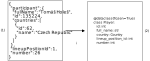
\includegraphics[width=0.9\textwidth]{../img/data_player.pdf}}
	\caption{Transformation of entity \emph{Player} from JSON to a Python class.}
	\label{fig:player}
\end{figure}

Entity {Player} is transformed from its initial JSON representation (\figref{player} - 1) to a easy-to-work-with Python's immutable class \emph{Player} with corresponding attributes. Note that a country has also a proper class \emph{Data.Country}.

\begin{figure}[h]
	\centering{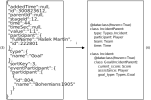
\includegraphics[width=1\textwidth]{../img/data_incident.pdf}}
	\caption{Transformation of entity \emph{Incident} from JSON to a Python class.}
	\label{fig:incident}
\end{figure} 

Entity \emph{Incident} is transformed from JSON (\figref{player} - 3) to a representation as an immutable Python's class (\figref{player} - 4). The class is called \emph{Goal} and it is a subclass of \emph{Incident}. This particular class structure ensures class addressing different types of incidents (goal/card/substitution/penalty kick) as one variable type and therefore enabling the \textit{Data.Match} class to have attribute \textit{incident} storing incidents as \emph{List[Incident]}. Furthermore, every \textit{Incident} subclass also inherits from \emph{IncidentParent} class since these are common attributes for every match incident and it would be inefficient to repeat those attributes multiple times.

Note that this module resolves part of content determination since number of attributes from initial JSON file are not transformed into Python class. For instance starting time of the match was not saved since I personally mark this information as redundant for a article generating. Similarly, more attributes were omitted to avoid useless information. On the other hand, couple attributes end up redundant (e.g. \textit{Country} of \textit{Player}), but these attributes are kept to ensure integrity of the solution and enabling easier further future development. 

\subsection{Document planner}

The aim of this module is to plan the content of the separate messages and their order. Document planner is resolved trivially - each incident is transformed to a separate preverbal message along with fundamental data. 

Implementation is shown in \figref{message} and is similar to Incident structure. Each preverbal message has different arguments and therefore own class. To access messages classes as one variable type there is a system of inheritance, where every message class inherits from \textit{MessageParent} so that they can be distinguished by their according type \textit{Types.Message}. Note that these classes again immutable to ensure data stability.

Unlike message class \textit{Substitution}, which is self-explanatory, classes \textit{Result} and \textit{MissedPenalty} need clarification. 

\textit{Result} message defines the title of the article. The core purpose of the title is to summarise a match in one sentence and hence to report the result/score of the match. 

Content of the \textit{MissedPenalty} is rather obvious, but the reasoning behind the existence of this separate class may not be visible at first glance and relies heavily on domain knowledge. Penalty is a crucial, rare and thrilling event during a football match.\footnote{Remember the famous penalty by Antonín Panenka in European Championship finals in 1976 that led to triumph of Czechoslovakia. The kick was groundbreaking and nowadays term 'Panenka' refers to a style of kick, where you only chip the ball in the middle of the net.} Consequently, every penalty is worth mentioning regardless of the outcome. However, if the penalty is successful the outcome is a goal and we would like to treat the message the same as any other goal. I believe every goal in a football match should be reported since scoring in football is rarer than in other sports in general (compared e.g. to basketball where reporting every basket would be too specific and unnecessary). Contrastingly, the message that reports a missed penalty is not required to be present in the article as this event did not affect the result directly and creates rather a shocking element of the article as players are expected to score from this position. This paragraph further illustrates the hand-crafted principles based on the domain knowledge that are incorporated in the solution.

\begin{figure}[h]
	\centering{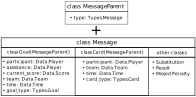
\includegraphics[width=1\textwidth]{../img/message_implementation.pdf}}
	\caption{Implementation of preverbal messages.}
	\label{fig:message}
\end{figure} 

\subsection{Sentence planner}
Last but not least is a sentence planner, that combines sentence aggregation, lexicalization and REG. Due to possible low number of messages to convey depends heavily on the course of the game, sentence aggregation is not performed. To further simplify process one incident corresponds to one sentence.

The core idea is to exploit method of templates, which is inserting words to express constituent (e.g. entities to be expressed from non-verbal message) verbally in the reserved empty spot in the sentence. However, to ensure some kind of variability as well as easy cooperating with Genja API the templates are resolved in a bit more complex way. Naming classes and variables throughout sentence planner was difficult due to the similarities of the segments that needed to be named, therefore I first present crucial classes and reveal their principle.

Firstly, the template, by its very nature, is represented as a class called \textit{\textbf{Sentence}}. \textit{Sentence} controls the structure of the sentence and allow other components of the implementation to insert various lexical items. \textit{Sentence} contains string \textit{id} to simplify number of types and subtypes in this section. Boolean \textit{simple} says whether the expression is simple, clear, syntactically easy or the opposite: colourful, longer and more complex. Then there is list of \textit{constituents}, which is either a hand-inserted string or \textit{Constituent}, that requires further development and will be picked later. Note that \textit{Sentence} consists attribute \textit{msg}, but the attribute is not assigned immediately.
\begin{Verbatim}[frame=single]
class Sentence:
	id: str
	simple: bool
	constituents: List[Union[str, Constituent]]
	msg: dp.Message
\end{Verbatim}
Here is an example of one \textit{Sentence} initialization, which defines the easiest possibility how to express a message that a goal was scored. Furthermore, following table shows possible lexicalization of these constituents in English(EN) and Czech(CZ) to illustrate the principle of such a structure.\footnote{Note that the order of the words is not correct in English, but correct in Czech. My translation will mainly illustrate the process for English readers, which can lead to grammatically incorrect sentences or expressions.}

\begin{Verbatim}[frame=single]
Sentence.create(type_, subtype, True, [
  Constituent(id_='e-time', morph_params='',
  	explicit_data=Types.ExplicitEntityData.TIME),
  Constituent(id_='v-goal', morph_params='.-0-.-.-.',
  	explicit_data=None),
  Constituent(id_='e-player', morph_params='1-.-0-.-.',
  	explicit_data=Types.ExplicitEntityData.PARTICIPANT),
  Constituent(id_='w-goal', morph_params='4-.-.-.-.',
  	explicit_data=None)]))
\end{Verbatim}

\begin{center}
	\begin{tabular}{ |c|c|c|c|c| }
		\hline
		 & Time & Verb for goal &Player entity &Word for goal \\ \hline
		 & e-time & v-goal & e-player & w-goal \\ \hline
		EN &In 7th minute& scored & Ronaldo & goal. \\  
		CZ & V 7. minutě & dal & Ronaldo & gól.\\
		\hline
	\end{tabular}
\end{center}

Another class is \textit{\textbf{Constituent}} containing again \textit{id} to mark its type or subtype. In Czech multiple agreements as well as grammatical cases need to be resolved and therefore we have to store such information when creating sentence layout regardless of the lexical expression that will be inserted. All morphology attributes are stored in \textit{morph\_params} containing case, tense, gender and ref/agr all to be then handed over to Genja API for linguistic realisation. Again, as seen in the \textit{Sentence} initialization, \textit{morph\_params} are initialized using string \textit{id}.

\begin{Verbatim}[frame=single]
class Constituent:
	id: str
	morph_params: MorphParams
	explicit_data: Types.ExplicitEntityData   
	string: str   
\end{Verbatim}

Lastly, class \textit{\textbf{Template}} handles the last step: how to lexicalize a constituent. 
\begin{Verbatim}[frame=single]
class Template:
	id: str
	string: str
\end{Verbatim}
\textit{Templates} can be strings, or a part of entity information can be inserted into a lexical item. \textit{Template}'s string can be defined by hand, or by function or by creating a template (by combining string and variables), which expresses the constituent. Here are examples for templates that express player entity and a word for assistance.

\begin{center}
	\begin{tabular}{ |c|c|c| }
		\hline
		\multicolumn{3}{| c |}{Entity player (e-player)} \\ \hline
		String for template & EN & CZ \\ \hline
		player.full\_name & Cristiano Ronaldo  & Cristiano Ronaldo \\
		player.get\_last\_name() & Ronaldo & Ronaldo \\
		"hráč číslo \$player.number" & player number 7 & hráč číslo 7 \\
		\hline
	\end{tabular}
\end{center}

\begin{center}
	\begin{tabular}{ |c|c| }
		\hline
		\multicolumn{2}{| c |}{Word assistance (w-assistance)} \\ \hline
		 EN & CZ \\ \hline
		assistance  & asistence\\
		pass & přihrávka \\
		\hline
	\end{tabular}
\end{center}

To recapitulate, class \textit{Sentence} creates templates for sentence combining and ordering numerous constituens, which are either hand-written string or represented as internal \textit{Constituent} class. For every \textit{Constituent} an instance of the class \textit{Template} is created to then present options for expressing \textit{Constituent} numerous ways.

To manage these objects and enable their cooperating, two handlers are created: \textit{SentenceHandler} and \textit{TemplateHandler}. \textit{Sentences} are first initialized all, then randomly shuffled and lastly grouped by their id and always using simple sentence first. Then for each message in the article a \textit{Sentence} is picked in the order they were grouped and message is assigned to the \textit{Sentence} as attribute \textit{msg}. Once every \textit{Sentence} for given message type is used, we pick randomly from used. This process ensures structural variability as we use same \textit{Sentence} twice only in case that we used all of the \textit{Sentences} for a given message.

To further increase variability of the created sentences similar process is repeated for \textit{Templates}. \textit{Templates} are randomly picked from non-used options. Once every template is present in the output, we pick random from every template ensuring we do not use same template twice in a row.

\subsection{Linguistic realiser}
Czech language is quite a complex language and therefore resolving the problem of realising chosen lexical items correctly by-hand without a proper tool performing complex morphology transformations is not efficient. This is the last step of the entire NLG, however, without the realisation the outputted text will not be readable. Therefore other software was used in order to perform linguistic realiser.

The system is called Genja provided by Geneea. Genja system, which was based on Jinja, operates with smart templates. In order to work with templates efficiently, Genja offer tools for managing morphology and knowledge base. Note that authorization key is required in order to perform linguistic realisation. This key stored as system environment variable to not be visible in a public GitHub repository. I would once more like to thank my supervisor for this possibility.

Due to the strict syntax that need to be inputed in a Genja API request, number of transformations need to be done. Firstly, combining plain string in a template with morphological parameters creating a well-built input for Genja. Secondly, json file for Genja must be created and lastly the output must be transformed from json back to string.

\subsection{Articles generator}
To finalize, articles generator connects modules together creating a notional one-way pipeline. 

\section{Output}
Since the lexical items are picked randomly, the output can contain sentences that are suboptimal and hard-to-read. For example when describing substitution message, realisation of two player entities can result in unappealing text, where it is not clearly visible who is the first and second player:
\begin{center}
	\textit{V 74. minutě střídal Vodháněl Kratochvíla Miloše.(CZ)}
	\textit{In 74th minute subbed Vodháněl Kratochvíla Miloše.(EN)}
\end{center}
Moreover, due to the international nature of football domain, often finding grammatically correct form of foreign name is not easy and Genja can not resolve this issue. 

To compensate these minor problems we output multiple texts instead of just one. As said, randomness can highly effect the overall impression from the text. When generating multiple texts the probability that one output will feel better than others is then increased. The idea of generating more than one text and then picking the best result of all generated can be useful, when the quality of the outputted text can not be ensured. However, the process of picking "the best" result can be again approached differently. For instance, using a human evaluation. Another option is to exploit the data-driven methods and pick the version that is statistically the most similar to the texts in acquired set of e.g. football articles from websites. The problem of selecting "the best" option is not solved in this project. 

Here is an example of lexicalization and realisation of one preverbal message:


As you can see the template system used created a variety of sentences.


Celé zápasy:

\section{Discussion}
In this section we discuss numerous perspectives and aspects of the solution.

First to discuss is the choice of the approach. The implementation strictly follows the division described in modular approach exploiting the power of splitting the extremely complex NLG problem into smaller easier-to-manage segments. As discussed earlier, the raw power of data can contribute to the quality of the result and therefore the first improvement of the project would be to change approach completely supposed you acquire the corpus data. However, stochastic approach rely on big amount of quality data, which are not available for me or rather their requirement would be insanely time-consuming. Moreover, this was my personally first NLG project. Due to my inexperience and lack of large number of easily accessible data the modular approach was chosen.

Naturally, quality of football articles created by sport journalists can hardly be matched with quality of outputs from the FootballArticlesGenerator software. The aim of the outputs were to be readable and form a proper Czech sentence filled with information about a football match, which was achieved. What is more, an increased variability was achieved to make text more fluid.

The complexity of the implementation was hard to deal with and not seeing the error propagation consequences the attempts of creating fully functioning system often failed. Retrospectively, the incorporated system of "two-layered" templates (implemented as \textit{Sentence} and \textit{Template}, which both fit to the template idea) is not-optimal. As seen in initializing \textit{Templates} for \textit{Time}. Firstly, the templates are picked randomly without context, meaning we can use expressions like "Two minutes after that" and so on. Secondly, to express time more variably we would like to use another template layer connected to a set of morphological parameters to be passed to Genja, but that is not possible. The best improvement for this project would be to re-implement sentence planner and using tree structure of templates to enable having template in a template. 

Such a tree structure would then require some non-trivial design and implementation to deliver the expected result. Sentences represented as trees where nodes are either strings or templates should be pre-created  to ensure variability between the sentences used throughout the text. Then the sentence aggregation can be performed once the content of the sentences is known. Lastly, lexicalizing each template in the sentence tree by various expressions. The core problem when designing this system is interconnection between the tasks, that requires a decent amount of flexibility of the tree structure in terms of implementation.  

Consequence of the well-implemented tree structure would be a better quality article. Due to the kept approach of using templates, the level of the result would not still be near to texts produced by humans. Templates offer only a number of varieties in comparison to a complex human language. Naturally, the higher the number of templates the more variable the text will be, initially approaching the human-like level. 

In addition, the database used for this project does not contain enough information to create somewhat complex article. Primary insufficiency is in the lack of details of incidents contained in the data. Expressing a goal is usually accompanied by a slight description of how the goal was scored: cross from the left side and top corner header, chaos in front of the net resulted in a rebound and a goal, beautiful solo play, 30 meter absolute screamer, etc. Similarly, the minor incidents like corners, shots, fouls, offsides are not present and could help when conveying more detailed text describing the true course of the game and not only major incidents. Lastly, there are no statistics and knowledge base present. When lexicalizing Cristiano Ronaldo we have only options to use number or name, while journalist would use more complicated expressions like "deadly portuguese striker", "famous CR7", "the most productive player of the Premiere League or "the newest member of Manchester United squad". History of the player, current leaderboards and statistics of the season, all time best leaderboards, nicknames for entities and more are the information lacking to truly have potential to create human-like article that would be both thrilling and informative. Not to mention incidents, which are not based on statistics, but rather on the actions that happened on the pitch. For instance, controversial calls, conflicts between players, vibes on the stadium, how well the team actually plays are all aspects that are very hard to store, classify and express, but are arguably the most interesting for a football fan besides a result of the match itself. This paragraph further proves the strength of the data-driven approach that can overcome the difficulties of lack of data by simply imitating the already existing text. For example, if corpus contains nickname "Blues" for "FC Chelsea" numerous times, it becomes a viable lexical expression for Chelsea entity.

Several papers on the topic of football summary or article were published...































\chapter*{Conclusion}
\addcontentsline{toc}{chapter}{Conclusion}
The aim of this thesis was to implement an NLG system that generates football articles from non-linguistic data. Along with the implementation, a brief NLG overview was required in order to have baseline knowledge for creating the intended software. We described the process of developing an NLG system end-to-end with tasks that are needed to take into consideration in order to create a fully functioning solution. We have covered the basics of NLG such as different approaches and their core benefits and drawbacks. Moreover, we have illustrated numerous problems that can arise during the development and that are required to be dealt with beforehand.

In the second section we present an implementation of such a text-generating system that uses slightly outdated (for reasons stated throughout the thesis multiple times), but, on the other hand, accessible methods. The implementation is described in detail. Choices made across the solution are usually explained as well. To inspect the implementation even more, please look into the code itself.

As stated in the end of the previous section, this work may not have that many implications. Although software can be used to present the course of the match in a textual and less-schematic representation, the quality of the outputted text is not on the newspaper level (which was not expected). Another problem with incorporating this project into other systems is the specificity of the input and the usage of linguistic realiser Genja, which is not available to the public. However, pieces in between said segments can be used. What is more, this paper can be utilised by other computer scientists, who lack complex insight into the field of computational linguistics and would like to study the subfield of NLG, since the overview of NLG is written from the perspective of a beginner. Furthermore, the text is filled with easy-to-follow examples and possible obstacles during the development to further illustrate knowledge carried across the paper. 


%%% Bibliography
\include{bibliography}

%%% Figures used in the thesis (consider if this is needed)
\listoffigures

\openright
\end{document}
